%-------------------------------------------------------------------------
\section{Introduction}
%-------------------------------------------------------------------------
L'objectif de ce document est de présenter la démarche 
suivie pour répondre aux exercices qui accompagnent le cours 
d'«~\href{http://www.enib.fr/~tisseau/pdf/course/info-S1.pdf}{Initiation à l'algorithmique}~» 
du semestre S1 à l'Ecole nationale d'ingénieurs de Brest (\enib). 
Cette démarche, dite \textsc{Mrv} (Méthode-Résultat-Vérification), est structurée en 3 étapes : 
\begin{enumerate}
\item on commence par expliciter la méthode générique qui permet de résoudre 
	des problèmes équivalents à celui qui est posé 
	(étape M comme Méthode);

\item on applique ensuite cette méthode générique au cas particulier de l'énoncé 
	pour obtenir le résultat attendu par l'exercice 
	(étape R comme Résultat);

\item enfin, on réalise une vérification du résultat obtenu à l'aide de techniques
	alternatives ou complémentaires connues
	(étape V comme Vérification).
\end{enumerate}
Pour fixer les idées, nous illustrons d'abord la démarche \textsc{Mrv} par deux exemples « simples »
(section \ref{sec:exemples}) : le passage des n\oe uds « marins » en 
kilomètres par heure « terrestres » (\ref{subsec:noeuds}) et
le calcul d'une fonction composée de segments de droite (\ref{subsec:fonction}).
Puis nous commentons quelques retours d'expériences (section \ref{sec:retours})
qui nous ont guidés dans l'élaboration de la démarche \textsc{Mrv} :
ne pas se tromper d'objectif (\ref{subsec:objectif}), expliciter l'implicite 
(\ref{subsec:qualite}) et encourager la rédaction (\ref{subsec:redaction}).
Forts de cette expérience, nous précisons ensuite les attendus à chaque étape
de la démarche \textsc{Mrv} (section \ref{sec:generalisation}) :
l'explicitation de la méthode (\ref{subsec:methode}), 
l'application de la méthode (\ref{subsec:resultat})
et la vérification du résultat (\ref{subsec:verification}).
Enfin, nous détaillons sa mise en \oe uvre (section \ref{sec:application})
à l'\enib{} dans le cadre du cours «~Initiation à l'algorithmique~» (\ref{subsec:contexte})
où elle conduit à une triple évaluation des exercices selon 
une notation adaptée (\ref{subsec:mrv}) dans le cadre d'un contrôle continu systématique
(\ref{subsec:cc}).

%-------------------------------------------------------------------------
\section{Exemples}\label{sec:exemples}
%-------------------------------------------------------------------------

Les exemples décrits dans cette section sont extraits des 
«~\href{http://www.enib.fr/~tisseau/pdf/course/q-info-S1.pdf}{Questionnements de cours}~»
qui complètent le cours d'Informatique S1 à l'\enib.
Chaque exemple est structuré ici en cinq paragraphes : 
\begin{enumerate}
\item l'objectif thématique de l'exercice,
\item l'énoncé de l'exercice,
\item la méthode générique utilisée pour résoudre une famille de problèmes 
	équivalents à celui de l'exercice proposé, 
\item le résultat obtenu en appliquant la méthode générique au cas particulier de l'énoncé,
\item la vérification du résultat.
\end{enumerate}

%-------------------------------------------------------------------------
\subsection{Des n\oe uds aux kilomètres par heure}\label{subsec:noeuds}
%-------------------------------------------------------------------------
\paragraph{Objectif} Mettre en \oe uvre l'instruction d'affectation.

\paragraph{Enoncé}
On veut convertir une certaine quantité $n1$ de vitesse exprimée en n\oe uds 
(miles nautiques par heure) en la quantité équivalente $n_2$ exprimée en 
kilomètres par heure (km/h).\\
Proposer une instruction de type « affectation » qui réalise cette conversion.

\paragraph{Méthode}
On cherche ici à convertir $n_1\cdot u_1$ en $n_2\cdot u_2$ 
où $u_1$ et $u_2$ sont des unités physiques compatibles 
qui dérivent de la même unité de base $u_b$ du \href{http://www.bipm.org/fr/si/}{Système international d'unités}.
$$\left|\begin{array}{l@{\ =\ }r}
u_1 & a_1\cdot u_b \\
u_2 & a_2\cdot u_b
\end{array}\right.
\ \Rightarrow\ \ 
\left|\begin{array}{l@{\ =\ }r@{\ =\ }r}
n_1\cdot u_1 & n_1\cdot (a_1\cdot u_b) & (n_1\cdot a_1)\cdot u_b\\
n_2\cdot u_2 & n_2\cdot (a_2\cdot u_b) & (n_2\cdot a_2)\cdot u_b
\end{array}\right.
\ \Rightarrow\ \ \frac{n_1\cdot u_1}{n_2\cdot u_2} = \frac{n_1\cdot a_1}{n_2\cdot a_2}$$
Comme on cherche $n_2$ tel que $n_1\cdot u_1 = n_2\cdot u_2$, on a donc :
$$\frac{n_1\cdot u_1}{n_2\cdot u_2} = \frac{n_1\cdot a_1}{n_2\cdot a_2} = 1
\ \Rightarrow\ \ n_2 = n_1 \cdot \frac{a_1}{a_2}$$
où les coefficients $a_i$ sont documentés dans le Système international d'unités par le
\href{http://www.bipm.org/}{Bureau international des poids et mesures}.

Une fois connus les coefficients $a_i$, on détermine la quantité $n_2$ de l'unité $u_2$
par une affectation simple : \texttt{n2 = n1*a1/a2} .

\paragraph{Résultat} On applique la méthode précédente à la conversion
proposée dans l'énoncé où $u_1$ représente les n\oe uds (miles nautiques par heure), 
$u_2$ les kilomètres par heure (km/h) et $u_b$ les mètres par seconde (m/s).
Le Système international d'unités fournit par ailleurs les facteurs 
de conversion $a_1$ (nd $\rightarrow$ m/s) et $a_2$ (km/h $\rightarrow$ m/s) :
$a_1 = 1852/3600$ et $a_2 = 1000/3600$.


\noindent\begin{minipage}[t]{7cm}
Compte-tenu de ces valeurs, le code ci-contre
permet de calculer le nombre $n_2$ de kilomètres par heure
en fonction du nombre $n_1$ de n\oe uds.
\end{minipage}
\hfill
\begin{minipage}[t]{8cm}
\begin{lstlisting}
a1 = 1852/3600
a2 = 1000/3600
n2 = n1*a1/a2
\end{lstlisting}
\end{minipage}

Remarque : on n'a pas cherché à effectuer « à la main » les calculs numériques :
\python{} les fera mieux que nous; et surtout, on n'a pas cherché non plus à 
particulariser la $3^{\grave eme}$ ligne du code en \texttt{n2 = n1*1852/1000} :
la forme plus abstraite \texttt{n2 = n1*a1/a2} restera identique pour convertir 
des parsecs en années-lumière (longueurs), des gallons en barils (volumes) ou 
encore des électron-volts en frigories (énergies), seules les valeurs des coefficients $a_i$ changeront (lignes \texttt{1} 
et \texttt{2} du code).

\paragraph{Vérification}
Pour tester le résultat précédent, on peut comparer les valeurs obtenues par le calcul 
avec celles de quelques valeurs caractéristiques facilement évaluables « à la main »
(exemples : $n_1 = 1\ \rm{nd} \Rightarrow{} n_2 = 1.852\ \rm{km/h}$ ou
$n_1 = 1/1852\ \rm{nd} \Rightarrow{} n_2 = 1/1000\ \rm{km/h}$).
$$\begin{minipage}[t]{7.5cm}\footnotesize
\begin{Verbatim}
>>> n1 = 1
>>> a1, a2 = 1852/3600, 1000/3600
>>> n2 = n1*a1/a2
>>> n2
1.852
\end{Verbatim}
\end{minipage}
\hfill
\begin{minipage}[t]{7.5cm}\footnotesize
\begin{Verbatim}
>>> n1 = 1/1852
>>> a1, a2 = 1852/3600, 1000/3600
>>> n2 = n1*a1/a2
>>> n2
0.0010000000000000002
\end{Verbatim}
\end{minipage}$$
On obtient bien par le calcul les résultats escomptés.

%-------------------------------------------------------------------------
\subsection{Graphe d'une fonction continue affine par morceaux}\label{subsec:fonction}
%-------------------------------------------------------------------------
\paragraph{Objectif} Mettre en \oe uvre l'instruction d'alternative multiple.

\paragraph{Enoncé}
On considère dans $\mathbb{R}$ la fonction continue $f$, affine par morceaux,  
définie sur $[-5;5]$  par le graphe ci-dessous et $\forall x < -5, f(x) = f(-5)$
et $\forall x > 5, f(x) = f(5)$. 
$$\begin{minipage}{6.75cm}
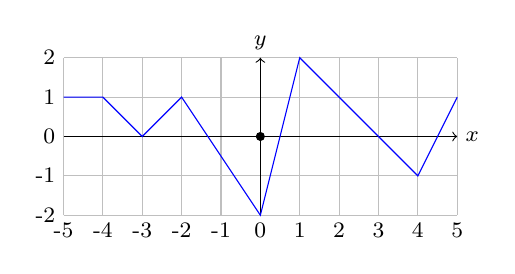
\begin{tikzpicture}[scale=0.5]\footnotesize
\draw[color=lightgray](-5,-2) grid[xstep=1,ystep=1] (5,2);
\foreach \x in {-5,-4,...,5} \draw(\x,-2) node[below]{\x};
\foreach \y in {-2,-1,...,2} \draw(-5,\y) node[left]{\y};
\filldraw(0,0) circle (0.1);
\draw[->] (-5,0) -- (5,0);
\draw (5,0) node[right]{$x$} ;
\draw[->] (0,-2) -- (0,2);
\draw (0,2) node[above]{$y$};
\draw[color=blue] (-5,1) -- (-4,1) -- (-3,0) -- (-2,1) -- (0,-2) -- (1,2) -- (4,-1) -- (5,1);
%\draw (-4.5,1) node[above]{\Pisymbol{pzd}{172}};
%\draw (-3.5,0.5) node[above]{\Pisymbol{pzd}{173}};
%\draw (-2.5,0.5) node[below]{\Pisymbol{pzd}{174}};
%\draw (-1,-0.5) node[below]{\Pisymbol{pzd}{175}};
%\draw (0.5,0) node[right]{\Pisymbol{pzd}{176}};
%\draw (2.5,0.5) node[right]{\Pisymbol{pzd}{177}};
%\draw (4.5,0) node[above]{\Pisymbol{pzd}{178}};
\end{tikzpicture}
\end{minipage}
$$
Proposer une instruction de type « alternative multiple » qui calcule la fonction $y = f(x)$
$\forall x \in \mathbb{R}$.

\paragraph{Méthode}
Il s'agit de déterminer la valeur $y = f(x)$ d'une fonction continue affine par morceaux sur $\mathbb{R}$. L'axe des réels $]-\infty,x_1,x_2,\ldots,x_n,+\infty[$ est donc vu comme une
succession d'intervalles $]-\infty,x_1[$, $[x_1,x_2[$, \ldots, $[x_{n-1},x_n[$ et
$[x_n,+\infty[$ sur lesquels la fonction $f$ est définie respectivement par les fonctions $f_1$, $f_2$, \ldots, $f_n$ et $f_{n+1}$ :
$$\begin{tabular}{l@{ $=$ }l@{ $\forall x \in$ }l}
$y = f(x)$ 	& $f_1(x)$		& $]-\infty,x_1[$ \\
			& $f_2(x)$ 		& $[x_1,x_2[$ \\
			& $f_3(x)$ 		& $[x_2,x_3[$ \\
			& \multicolumn{2}{l}{\ldots} \\
			& $f_n(x)$ 		& $[x_{n-1},x_n[$\\
			& $f_{n+1}(x)$ 	& $[x_n,+\infty[$
\end{tabular}$$
Chacune des fonctions $f_i$ correspond à une droite d'équation $y = a_ix+b_i$ où $a_i$
représente la pente de la droite et $b_i$ son ordonnée à l'origine.
Lorsqu'on connaît 2 points $M(x_M,y_M)$ et $N(x_N,y_N)$ 
d'une droite d'équation $y = ax + b$, les coefficients $a$ (pente de la droite) 
et $b$ (ordonnée à l'origine) de la droite sont obtenus
par résolution du système de 2 équations : $y_M =ax_M + b$ et $y_N = ax_N + b$. 
On obtient alors $a$ et $b$ :

$$\begin{minipage}{6.75cm}
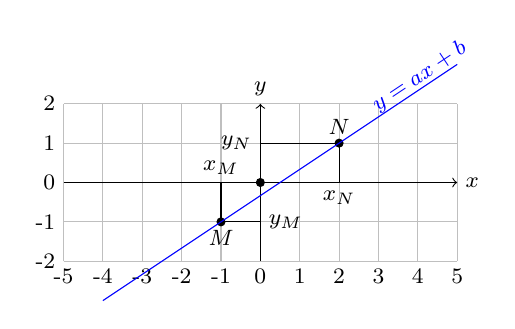
\begin{tikzpicture}[scale=0.5]\footnotesize
\draw[color=lightgray](-5,-2) grid[xstep=1,ystep=1] (5,2);
\foreach \x in {-5,-4,...,5} \draw(\x,-2) node[below]{\x};
\foreach \y in {-2,-1,...,2} \draw(-5,\y) node[left]{\y};
\filldraw(0,0) circle (0.1);
\filldraw(-1,-1) circle (0.1);
\draw (-1,-1) node[below]{$M$};
\draw(-1,0) node[above]{$x_M$};
\draw(0,-1) node[right]{$y_M$};
\draw (-1,-1) -- (-1,0);
\draw (-1,-1) -- (0,-1);
\filldraw(2,1) circle (0.1);
\draw (2,1) node[above]{$N$};
\draw(2,0) node[below]{$x_N$};
\draw(0,1) node[left]{$y_N$};
\draw (2,1) -- (2,0);
\draw (2,1) -- (0,1);
\draw[->] (-5,0) -- (5,0);
\draw (5,0) node[right]{$x$} ;
\draw[->] (0,-2) -- (0,2);
\draw (0,2) node[above]{$y$};
\draw[color=blue] (-4,-3) -- (5,3);
\draw[color=blue](4.3,2.3) node[above,rotate=33.69]{$y = ax + b$};
\end{tikzpicture}
\end{minipage}
\hfill
\begin{minipage}{8.75cm}
$$\displaystyle a = \frac{y_N - y_M}{x_N - x_M} \mbox{ et } \displaystyle b = \frac{y_Mx_N - y_Nx_M}{x_N - x_M}$$
Pour la droite ci-contre :
$$\displaystyle 
a = \frac{1 - (-1)}{2 - (-1)} = \frac{2}{3} \mbox{ et } \displaystyle 
b = \frac{(-1)\cdot 2 - 1\cdot(-1)}{2 - (-1)} = -\frac{1}{3}
$$
On vérifie graphiquement ces résultats : pour passer de $M$ à $N$, on
se déplace de $\Delta x = 3$ horizontalement puis de $\Delta y = 2$ verticalement 
(d'où la pente $a = \Delta y/\Delta x = 2/3$),
et la droite coupe bien l'axe des ordonnées en $y = -1/3$.
\end{minipage}$$
Une fois déterminés les coefficients $a_i$ et $b_i$ de chaque droite, on détermine
la valeur de la fonction $y = f(x)$ par une alternative multiple du genre :
$$\begin{minipage}{5.5cm}\tt
if   x < $x_1$ : y = $a_1$*x + $b_1$\\
elif x < $x_2$ : y = $a_2$*x + $b_2$\\
elif x < $x_3$ : y = $a_3$*x + $b_3$\\
...\\
elif x < $x_n$ : y = $a_n$*x + $b_n$\\
else           : y = $a_{n+1}$*x + $b_{n+1}$
\end{minipage}$$

\paragraph{Résultat} On applique la méthode précédente à la fonction $f$ de l'énoncé.
Il faut donc déterminer les équations de droite 
correspondant aux différents segments du graphe de la fonction, à savoir :
$$\begin{minipage}{9cm}
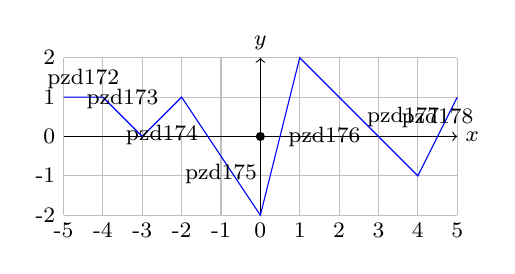
\begin{tikzpicture}[scale=0.5]\footnotesize
\draw[color=lightgray](-5,-2) grid[xstep=1,ystep=1] (5,2);
\foreach \x in {-5,-4,...,5} \draw(\x,-2) node[below]{\x};
\foreach \y in {-2,-1,...,2} \draw(-5,\y) node[left]{\y};
\filldraw(0,0) circle (0.1);
\draw[->] (-5,0) -- (5,0);
\draw (5,0) node[right]{$x$} ;
\draw[->] (0,-2) -- (0,2);
\draw (0,2) node[above]{$y$};
\draw[color=blue] (-5,1) -- (-4,1) -- (-3,0) -- (-2,1) -- (0,-2) -- (1,2) -- (4,-1) -- (5,1);
\draw (-4.5,1) node[above]{\Pisymbol{pzd}{172}};
\draw (-3.5,0.5) node[above]{\Pisymbol{pzd}{173}};
\draw (-2.5,0.5) node[below]{\Pisymbol{pzd}{174}};
\draw (-1,-0.5) node[below]{\Pisymbol{pzd}{175}};
\draw (0.5,0) node[right]{\Pisymbol{pzd}{176}};
\draw (2.5,0.5) node[right]{\Pisymbol{pzd}{177}};
\draw (4.5,0) node[above]{\Pisymbol{pzd}{178}};
\end{tikzpicture}
\end{minipage}
\hfill
\begin{minipage}{3cm}
\begin{itemize}
\item[\Pisymbol{pzd}{172}] $y = 1$
\item[\Pisymbol{pzd}{173}] $y = -x -3$
\item[\Pisymbol{pzd}{174}] $y = x + 3$
\item[\Pisymbol{pzd}{175}] $y = -3x/2 - 2$
\item[\Pisymbol{pzd}{176}] $y = 4x - 2$
\item[\Pisymbol{pzd}{177}] $y = -x + 3$
\item[\Pisymbol{pzd}{178}] $y = 2x - 9$
\end{itemize}
\end{minipage}$$

\noindent\begin{minipage}[t]{7cm}
Compte-tenu de ces équations, le code ci-contre
permet de calculer $y = f(x)$, y compris pour $x < -5$ ($y = f(-5) =1$) et 
$x > 5$ ($y = f(5) = 1$).

Remarque : on aurait pu simplifier les deux premières lignes de ce code en\\
\centerline{\texttt{if x < -4 : y = 1}}
car les instructions associées sont iden\-tiques (ie. les fonctions
affines sont identiques sur $]-\infty,-5[$ et $[-5,-4[$).
\end{minipage}
\hfill
\begin{minipage}[t]{8cm}\footnotesize
\begin{lstlisting}
if   x < -5 : y = 1
elif x < -4 : y = 1
elif x < -3 : y = -x - 3
elif x < -2 : y = x + 3
elif x <  0 : y = -3*x/2 - 2
elif x <  1 : y = 4*x - 2
elif x <  4 : y = -x + 3
elif x <  5 : y = 2*x - 9
else        : y = 1
\end{lstlisting}
\end{minipage}

\paragraph{Vérification} Pour tester le résultat précédent, 
on peut comparer les valeurs obtenues par le calcul avec celles lues
directement sur le graphe pour quelques points caractéristiques.
Ces points de mesure sont choisis judicieusement : ils ne correspondent 
pas aux bornes des intervalles déjà prises en compte dans la méthode
mais plutôt à des points où la fonction s'annule 
(exemples : $x = -4/3$, $1/2$, $3$ ou $9/2$)
ou à des points d'abscisses aux n\oe uds de la grille de lecture 
(exemples : $x = -1$ ou $x = 2$).
On peut vérifier par exemple pour $x = -1$ 
($y = f(-1) = -1/2$) et $x = 3$ ($y = f(3) = 0$).
$$\begin{minipage}{7.5cm}\footnotesize
\begin{Verbatim}
>>> x = -1
>>> if x < -4 : y = 1
elif   x < -3 : y = -x - 3
elif   x < -2 : y = x + 3
elif   x <  0 : y = -3*x/2 - 2
elif   x <  1 : y = 4*x - 2
elif   x <  4 : y = -x + 3
elif   x <  5 : y = 2*x - 9
else          : y = 1

>>> y
-0.5
\end{Verbatim}
\end{minipage}
\hfill
\begin{minipage}{7.5cm}\footnotesize
\begin{Verbatim}
>>> x = 3
>>> if x < -4 : y = 1
elif   x < -3 : y = -x - 3
elif   x < -2 : y = x + 3
elif   x <  0 : y = -3*x/2 - 2
elif   x <  1 : y = 4*x - 2
elif   x <  4 : y = -x + 3
elif   x <  5 : y = 2*x - 9
else          : y = 1

>>> y
0
\end{Verbatim}
\end{minipage}$$
On obtient bien par le calcul les résultats lus sur la grille.

%-------------------------------------------------------------------------
\section{Retours d'expériences}\label{sec:retours}
%-------------------------------------------------------------------------
Les exercices présentés précédemment (section \ref{sec:exemples})
ont été proposés à de nombreuses générations d'étudiants de l'\enib{}
bien avant d'utiliser la démarche \textsc{Mrv}. Les retours d'expériences
associés ont permis de mettre en évidence au moins trois
réflexions méthodologiques : 
ne pas se tromper d'objectif (\ref{subsec:objectif}),
expliciter l'implicite (\ref{subsec:qualite}) et
encourager la rédaction (\ref{subsec:redaction}).

%-------------------------------------------------------------------------
\subsection{Ne pas se tromper d'objectif}\label{subsec:objectif}
%-------------------------------------------------------------------------
Les étudiants de l'\enib{} sont issus des voies scientifique (\bac{} S)
et technique (\bac{} \sti) de l'enseignement secondaire. 
C'est pourquoi, pour donner du sens aux exercices d'algorithmique, 
de nombreux exemples sont empruntés aux mathématiques, à la physique 
et plus généralement aux sciences de l'ingénieur. 
C'est ainsi le cas des deux exemples précédents : la physique pour les
conversions d'unités (exercice \ref{subsec:noeuds}) et les mathématiques pour les
fonctions continues affines par morceaux (exercice \ref{subsec:fonction}).

Ces emprunts interdisciplinaires sont absolument nécessaires pour participer
au décloisonnement des disciplines\ldots{} que les étudiants ont progressivement 
appris à cloisonner et à isoler au cours de leur scolarité. 
Mais ils posent le problème de l'objectif thématique de l'exercice. 
En effet, les étudiants peuvent être si perturbés par la thématique 
secondaire (ici les mathématiques ou la physique) qu'ils en oublient la
thématique principale (ici l'algorithmique), ce qui n'est évidemment pas 
le but recherché par l'exercice d'algorithmique.

Dans l'exemple de la fonction continue affine par morceaux, un point de blocage
souvent rencontré porte sur la détermination de l'équation d'une droite. 
A ce niveau (premier semestre de l'enseignement supérieur), 
très peu d'étudiants en difficulté avec l'équation d'une droite,
«~oseront~» écrire quelque chose comme :
« supposons que l'on connaisse l'équation de la droite $y = f_i(x)$
dans l'intervalle $i$ considéré, alors l'alternative multiple recherchée 
s'écrira sous la forme\ldots{} ». Or, c'est pourtant fondamentalement ce qu'attend l'informaticien, quelle que soit sa «~déception~» face à la non-maîtrise d'une notion
mathématique aussi élémentaire que l'équation d'une droite.
Dans une initiation à l'algorithmique, on s'attachera à vérifier 
la cohérence logique des différentes conditions de l'alternative multiple 
plutôt que la précision des instructions associées à ces conditions. 
Ainsi, une réponse cohérente du point de vue des conditions de l'alternative
multiple sera beaucoup plus proche de l'objectif recherché qu'une réponse 
incohérente sur les conditions même avec des équations de droite correctes.

On s'attachera alors à expliciter l'objectif thématique de l'exercice et
à renseigner au mieux les éléments nécessaires aux thématiques secondaires.
On rappellera aux étudiants que l'évalua\-tion porte sur l'objectif thématique
principal et non sur les thématiques secondaires.


%-------------------------------------------------------------------------
\subsection{Expliciter l'implicite}\label{subsec:qualite}
%-------------------------------------------------------------------------
Si on retient que la qualité d'une réponse est son aptitude à satisfaire
strictement aux besoins exprimés dans la question, alors les étudiants de l'\enib{} sont 
devenus des professionnels de la qualité. 
Dans l'exemple de la conversion d'unités,
il est fréquent que la réponse des étudiants tienne en une seule ligne : 
\texttt{n2 = 1.852*n1}, ce qui est effectivement la bonne réponse qui 
mérite donc, dans leur esprit, la meilleure appréciation.
Mais si l'on peut se contenter de cette réponse dans un contexte de physique
élémentaire, il n'en va pas de même dans un contexte de formation d'ingénieur.

En algorithmique, on cherche à caractériser différentes propriétés d'un algorithme
telles que sa validité, sa réutilisabilité, sa robustesse, sa complexité 
ou encore son efficacité. Il faut donc progressivement développer chez 
l'informaticien débutant des réflexes de validation, de réutilisation, 
de protection, d'évaluation ou encore d'adaptation au support matériel.
L'acquisition de ces réflexes méthodologiques doit être évaluée au même titre
que l'acquisition des connaissances proprement dites comme l'affectation ou 
l'alternative multiple. Il faut donc expliciter auprès des étudiants ces objectifs méthodologiques et ne pas les cantonner au niveau d'objectifs implicites
plus ou moins pris en compte dans l'évaluation d'une réponse à un exercice donné.

En premier lieu, il faut s'assurer que l'algorithme est valide :
réalise-t-il exactement la tâche pour laquelle il a été conçu ?
On demandera alors explicitement aux étudiants de proposer une démarche 
de vérification de leurs réponses. 
Dans l'exemple de la fonction continue affine par morceaux, on compare le résultat
du calcul par algorithme à une lecture directe sur le graphe pour quelques points caractéristiques bien choisis (points où la fonction s'annule,  
points aux n\oe uds de la grille de lecture). Cette méthode ne permet évidemment
pas de valider l'algorithme $\forall x \in \mathbb{R}$, mais permet d'invalider
l'algorithme proposé s'il existe une incohérence entre le calcul et la lecture
directe sur le graphe pour un des points caractéristiques considérés.
Cette «~vérification~» n'en demeure pas moins satisfaisante, et essentielle, 
dans un cours d'initiation à l'algorithmique.

Dans un deuxième temps, on s'intéresse à sa généricité : l'algorithme
est-il réutilisable pour résoudre des tâches équivalentes à celle 
pour laquelle il a été conçu ?
Dans l'exemple de la conversion d'unités, on préfère l'affectation
générique (\texttt{n2 = n1*a1/a2}) à l'affectation particulière
(\texttt{n2 = n1*1852/1000}) et encore plus à l'affectation pré-calculée
(\texttt{n2 = 1.852*n1}). L'affectation générique s'applique en effet
à toute conversion d'unités linéairement dépendantes l'une de l'autre.
L'affectation particulière répond correctement mais de manière \emph{ad hoc} 
au problème posé, ce qui ne permet pas sa réutilisabilité à d'autres types d'unités,
y compris même à d'autres unités de vitesse telle que la conversion de miles terrestres
par heure en kilomètres par heure  ($1\ \mbox{mi} = 1.609344\cdot 10^3\ \mbox{m}$). Quant à l'affectation pré-calculée, outre le fait qu'on n'est jamais à l'abri d'une erreur de calcul, elle ne permettra pas de « remonter » 
aussi facilement que les deux autres à la signification du coefficient numérique calculé et
donc, ne facilitera pas la maintenance du code proposé.

Dans un troisième temps, on s'attachera à le rendre robuste : 
l'algorithme est-il protégé de conditions anormales d'utilisation ?
Dans l'exemple de la conversion d'unités, l'affectation générique \texttt{n2 = n1*a1/a2}
ne s'applique qu'à des unités linéairement dépendantes l'une de l'autre ($u_2 = \alpha u_1$).
Il existe cependant des grandeurs qui sont en relation affine l'une de l'autre 
($u_2 = \alpha u_1 + \beta$).
C'est le cas des températures \textsc{Farenheit} $t_F$ et \textsc{Celsius} $t_C$ qui sont reliées à la température thermodynamique \textsc{Kelvin} $T_K$ 
(unité de base des températures) 
par les relations $t_C =  T_K - 273.15$ et $t_F = 9T_K/5 - 459.67$, 
soit $t_C = 5/9\cdot(t_F + 459.67) - 273.15$ entre elles.
En algorithmique, l'étude des fonctions et de leurs préconditions (conditions d'application)
permettra d'aborder systématiquement cette propriété de robustesse.

En ce qui concerne les propriétés d'un algorithme telles que la complexité 
(combien d'instruc\-tions élémentaires seront exécutées pour réaliser la tâche pour 
laquelle l'algorithme a été conçu ?) et l'efficacité 
(l'algorithme utilise-t-il de manière optimale les ressources du matériel qui l'exécu\-te ?),
elles seront abordées au travers d'exemples précis, leur étude systématique ne relevant pas
du cours d'initiation à l'algorithmique de l'\enib.

Dans tous les cas, on s'attachera à préciser le ou les objectifs méthodologiques 
de l'exercice qui seront alors évalués explicitement au même titre que l'objectif thématique.

%-------------------------------------------------------------------------
\subsection{Encourager la rédaction}\label{subsec:redaction}
%-------------------------------------------------------------------------
La rédaction « en bon français » de la réponse à un exercice ne constitue pas le point 
fort des jeunes étudiants de l'\enib. Les réponses sont (trop) souvent libellées 
« simplement » sous forme de valeurs, de formules, de diagrammes ou de codes informatiques : 
aucune explication « en bon français » ne vient compléter ni expliciter la réponse, 
ni la démarche qui a conduit à cette réponse, encore moins la critique de la solution proposée.
Et pourtant, si la réponse à la question est attendue, les éléments de discours 
qui l'accompagnent le sont tout autant, d'autant plus dans une formation d'ingénieurs
qui vise à former des professionnels qui devront rédiger des cahiers des charges,
des spécifications et des conceptions détaillées, des recettes de tests, des notes
de synthèse, écrites comme orales, ou encore des réponses à des appels d'offres.
Le métier d'ingénieur ne peut se contenter d'une valeur, d'une formule, d'un diagramme 
ou d'un code : s'il faut être capable de trouver une solution à un problème donné,
il faut aussi savoir «~défendre~» rationnellement la solution proposée.
L'argumentaire qui accompagne la solution proposée doit permettre de mieux comprendre 
cette solution et augmenter ainsi la confiance du « lecteur » dans les compétences du
« rédacteur » à résoudre le problème posé.

On s'attachera alors à prendre en compte explicitement la rédaction dans
l'évaluation de la réponse. Il faudra sans doute pour cela, soit augmenter le temps
accordé à l'exercice, soit diminuer le nombre d'exercices à résoudre dans un temps 
imparti, pour permettre à l'étudiant « rédacteur » de soigner cet aspect important
de sa réponse.

%-------------------------------------------------------------------------
\section{Généralisation}\label{sec:generalisation}
%-------------------------------------------------------------------------

A l'aune des exemples précédents (section \ref{sec:exemples}) et des retours d'expériences associés (section~\ref{sec:retours}), 
cette section reconsidère les trois étapes de la démarche \textsc{Mrv} : 
explicitation de la méthode (\ref{subsec:methode}), 
application de la méthode (\ref{subsec:resultat}) et 
vérification du résultat (\ref{subsec:verification}).

%-------------------------------------------------------------------------
\subsection{Explicitation de la méthode}\label{subsec:methode}
%-------------------------------------------------------------------------
Etant donné un énoncé qui propose de résoudre un exercice
portant sur un cas particulier donné, la première étape de la démarche \textsc{Mrv} consiste à
décrire une méthode générique qui, lorsqu'on l'appliquera, permettra de résoudre 
le cas particulier considéré ainsi que tout problème équivalent à celui 
qui est posé.

Pour un débutant, cette étape d'explicitation d'une méthode générique est une étape  
difficile. Elle nécessite de développer des capacités 
d'abstraction qui mettent en \oe uvre des mécanismes d'induction 
pour favoriser le passage de données particulières à des propositions plus générales.
L'induction est en effet un type de raisonnement qui permet de «~remonter~»
de cas particuliers à la loi qui les régit, des effets à la cause ou encore des conséquences au principe.
% : elle génère ainsi du sens en passant du particulier au général.

C'est également une étape difficile parce que la description d'une méthode peut 
difficilement se résumer à une valeur, une formule, un diagramme ou un code
informatique.
Elle nécessite une phase rédactionnelle rigoureuse et suffisamment détaillée pour
qu'un lecteur averti puisse appliquer sans hésiter la méthode décrite.

Cette étape permet ainsi de développer des capacités d'abstraction et
des capacités rédactionnelles absolument nécessaires aux futurs ingénieurs.

%-------------------------------------------------------------------------
\subsection{Application de la méthode}\label{subsec:resultat}
%-------------------------------------------------------------------------
Etant donné une méthode générique pour résoudre un ensemble de problèmes 
équivalents, le deuxième étape de la démarche \textsc{Mrv} consiste à
appliquer cette méthode à un problème particulier.

Pour un débutant, cette étape d'application d'une méthode générique est une étape 
assez facile. Elle nécessite de développer des capacités d'exécution
qui mettent en \oe uvre des mécanismes de déduction pour réaliser le passage
de propositions générales à un cas particulier.
A l'inverse de l'induction, la déduction est en effet un type de raisonnement
qui « va » du général au particulier, de la cause aux effets ou encore du principe aux
conséquences.

Cette étape permet ainsi de développer des capacité d'exécution en respectant
rigoureusement des consignes imposées. Elle met ainsi en évidence des capacités 
« techniciennes » qui seront très utiles aux futurs ingénieurs dans leur mission 
d'encadrement d'équipes d'ouvriers et de techniciens.


%-------------------------------------------------------------------------
\subsection{Vérification du résultat}\label{subsec:verification}
%-------------------------------------------------------------------------
Etant donné un résultat obtenu par application d'une méthode générique pour résoudre un problème particulier, la troisième étape de la démarche \textsc{Mrv} consiste à vérifier ce résultat
par des méthodes alternatives ou complémentaires de celle déjà utilisée.

Pour un débutant, cette étape de vérification du résultat obtenu est assez difficile
car il s'agit avant tout de remettre en cause son propre travail. 
Dans le meilleur des cas, le débutant estime que la vérification consiste simplement 
à refaire les mêmes calculs, le même raisonnement ou la même démarche : 
c'est effectivement la moindre des choses que de ré-appliquer la méthode pour vérifier 
qu'on ne s'est pas trompé en l'appliquant la première fois. 
Mais la vérification consiste plutôt à changer de point de vue sur le problème
et à utiliser d'autres méthodes pour «~estimer~» la validité du résultat.

Il peut effectivement exister plusieurs méthodes alternatives pour résoudre un même
problème. Résoudre alors le problème par deux méthodes différentes et obtenir le 
même résultat renforce bien entendu la « confiance » en ce résultat.
Mais dans bien des cas, il s'agit plutôt de méthodes complémentaires, le plus souvent 
sous forme d'heuristiques, qui permettent de détecter que le résultat est 
certainement faux, comme par exemple la preuve par 9 en calcul élémentaire ou
l'analyse dimensionnelle en physique. Et si de telles méthodes complémentaires ne détectent pas que le 
résultat est faux, alors ça renforce ici encore la « confiance » que l'on peut
avoir dans le résultat obtenu.

Cette étape permet ainsi de développer l'esprit critique des futurs ingénieurs en 
insistant sur le souci de vérification systématique de ses propres résultats
comme de ceux provenant d'autres sources (collègues, articles, internet\ldots).

%-------------------------------------------------------------------------
\section{Mise en \oe uvre}\label{sec:application}
%-------------------------------------------------------------------------
La démarche \textsc{Mrv} est mise en \oe uvre dans le cours 
d'«~\href{http://www.enib.fr/~tisseau/pdf/course/info-S1.pdf}{Initiation à l'algorithmique}~» 
du semestre S1 à l'\enib{} (\ref{subsec:contexte}). 
Lors des contrôles, elle conduit à une triple évaluation des exercices 
selon une notation adaptée (\ref{subsec:mrv}) dans le cadre d'un contrôle continu 
systématique (\ref{subsec:cc}). 


%-------------------------------------------------------------------------
\subsection{Contexte}\label{subsec:contexte}
%-------------------------------------------------------------------------

Les «~\href{http://www.enib.fr/~tisseau/pdf/course/q-info-S1.pdf}{Questionnements de cours}~»
qui accompagnent le cours d'«~\href{http://www.enib.fr/~tisseau/pdf/course/info-S1.pdf}{Initiation à l'algorithmique}~» 
du semestre S1 à l'\enib{} sont conçus de façon plutôt «~ascendante~» (de l'exemple au concept) et se veulent 
complémentaires des notes de cours qui, elles, sont conçues plutôt classiquement
de façon «~descendante~» (du concept à l'exemple).

Chaque questionnement concerne un point particulier du cours; il
est structuré en 5 parties de la manière suivante :
\begin{enumerate}
\item Exemple : dans cette partie, des questions « simples » sont posées 
	sur un problème «~connu~» de la «~vie courante~» afin d'introduire 
	le concept informatique sous-jacent. On y trouvera des
	exemples tels qu'aller au restaurant,
		ranger un meuble à tiroirs,
		analyser les sorties d'un circuit logique,
		compter avec \textsc{Bobby Lapointe} en base «~bibi~»,
		déterminer sa mention au bac,
		planter un clou,
		ranger des rondins de bois,
		cuisiner un quatre-quarts aux pépites de chocolat,
		jouer aux tours de Hanoï ou encore
		trier un jeu de cartes.
		
		Cette partie est principalement traitée de manière informelle 
		par les étudiants eux-mêmes, individuellement ou en groupe.
		
\item Généralisation : dans cette partie, les concepts informatiques sous-jacents
	sont présentés et introduits à l'aide de questions plus «~informatiques~».
	On y aborde les concepts 
	d'algorithmique,
	d'affectation,
	de calculs booléens,
	de codage des nombres,
	de tests et d'alternatives,
	de boucles,
	de spécification de fonction ,
	de récursivité ou encore
    de manipulation de séquences.

	En général, cette partie est traitée par l'enseignant.
	
\item Applications : des exemples « simples » d'application sont ensuite proposés.

	Le premier exemple est en général traité \emph{in extenso} par l'enseignant
	en suivant la démarche \textsc{Mrv}, les autres
	par les étudiants, en groupe ou individuellement.
	
\item Entraînement : cette partie est une préparation à l'évaluation qui a lieu
	en début de séance suivante. Les étudiants y travaillent chez eux entre les deux séances, 		individuellement ou en groupe.
	
	\begin{enumerate}
 	\item Enoncé : on présente ici le problème que l'on souhaite traiter tel que
 			le calcul en base «~Shadok~»,
 			le calcul de facteurs de conversion entre unités physiques,
 			l'établissement de la table de vérité d'une expression logique,
 			l'écriture d'un nombre réel selon la norme \textsc{Ieee} 754,
 			la détermination de la valeur d'une fonction continue et linéaire par morceaux,
 			le calcul d'un développement limité selon une certaine précision,
 			le dessin d'un motif géométrique composé de polygones réguliers,
 			la spécification d'une fonction connue (un « grand classique » de la programmation),
 			le parcours d'un arbre binaire ou encore
 			le tri d'un annuaire selon différents critères.
 			
 	\item Exemple : un exemple est traité en détail dans cette partie en suivant la 
 		démarche \textsc{Mrv}. Ce sont de tels exemples qui ont été présentés dans la section
 		\ref{sec:exemples} du présent document.
 		
 	\item Questions : 24 questions de même difficulté sont proposées ici pour permettre 
 		à chaque étudiant de s'entraîner sur le problème à traiter. La résolution de 2 
 		ou 3 de ces exemples l'aide ainsi à induire (à faire émerger) la méthode générique qui
 		est attendue ainsi qu'à mener explicitement les vérifications souhaitées.
 		
 		Le jour de l'évaluation, chaque étudiant traite individuellement une des 24
 		questions tirée au sort le jour du contrôle (une question différente par élève). 
 		Lors de cette évaluation, tous documents, calculettes, téléphones et ordinateurs 
 		sont interdits.
 		A la fin de chaque contrôle, il est demandé à chaque étudiant de s'auto-évaluer 
		pour chacune des étapes de la méthode \textsc{Mrv} selon une grille de notation 
		à 4 niveaux (voir section \ref{subsec:mrv} suivante).
		Enfin, une correction est proposée par l'enseignant juste après le
		contrôle, « à chaud ».
 		
 	\end{enumerate}
\item Révisions : Cette partie fait le lien entre les questionnements de cours et les 
	notes de cours.
\end{enumerate}

%-------------------------------------------------------------------------
\subsection{Triple évaluation}\label{subsec:mrv}
%-------------------------------------------------------------------------
Chaque contrôle donne lieu a une triple évaluation de la part de l'enseignant : 
une évaluation concerne la qualité de l'explicitation de la méthode générique (M), 
une autre la qualité du résultat obtenu (R) et la troisième la pertinence de la 
vérification du résultat (V). Ainsi, le résultat à la question posée, dont se
contentent le plus souvent les étudiants, n'est plus le seul élément de réponse attendu :
il est également demandé aux étudiants d'expliciter la méthode utilisée ainsi
que les vérifications menées.

La grille de notation adoptée doit permettre de « soulager » l'enseignant 
dans sa tâche de correction et d'aider les étudiants à mener leurs propres évaluations. 
Un exercice cherchant à évaluer un objectif
particulier, la notation exprime alors « simplement » la distance qui reste à parcourir 
pour atteindre cet objectif. Quatre « distances » sont ainsi pré-définies selon
une métaphore de la cible : 
$$\begin{minipage}{11.75cm}%\footnotesize
\noindent\begin{tabular}{l@{ : }l@{ $\rightarrow$ }l}
0 & «~en plein dans le mille !~» & l'objectif est atteint \\
1 & «~pas mal !~» & on est proche de l'objectif \\
2 & «~juste au bord de la cible !~» & on est encore loin de l'objectif\\
3 & «~la cible n'est pas touchée !~» & l'objectif n'est pas atteint
\end{tabular}
\end{minipage}
\hspace*{5mm}
\begin{minipage}{3.25cm}
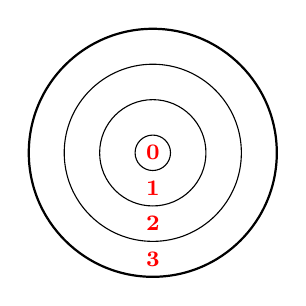
\begin{tikzpicture}[scale=0.45]\footnotesize
\draw (0,0) circle (0.5);
\draw (0,0) circle (1.5);
\draw (0,0) circle (2.5);
\draw[thick] (0,0) circle (3.5);
\node at (0,0) {\color{red}\textbf{0}};
\node at (0,-1) {\color{red}\textbf{1}};
\node at (0,-2) {\color{red}\textbf{2}};
\node at (0,-3) {\color{red}\textbf{3}};
%\draw (-3.5,-3.5) rectangle (3.5,3.5);
\end{tikzpicture}
\end{minipage}$$
Ayant choisi de ne garder qu'un petit nombre de niveaux pour « faciliter »
l'évaluation, le choix de 4 niveaux a finalement été préféré à 2, 3 ou 5 niveaux :
\begin{itemize}
\item une notation sur 2 niveaux (\emph{tout ou rien}) est un peu trop 
	caricaturale;
\item avec un (petit) nombre impair de niveaux (3 ou 5), l'expérience montre
	que, dans le doute, le correcteur a tendance à choisir plus facilement 
	le niveau du milieu (1 ou 3) alors qu'avec un nombre pair de niveau (ici 4), il
	doit « choisir son camp » : objectif plutôt atteint (0 ou 1) ou plutôt raté
	(2 ou 3).
\end{itemize}
En fait, il existe un cinquième niveau qui correspond à une absence au contrôle, 
sanctionnée par la note 4 (l'objectif n'a pas été visé), dite note minimale.	

Ainsi, et pour changer de point de vue sur la notation, le contrôle 
est réussi lorsqu'on a 0 ! Il n'y a pas non plus de $1/2$ point ou de $1/4$ 
de point : le seul barème possible ne comporte que 4 niveaux : 0, 1, 2 et 3.
On ne cherche donc pas à «~grappiller~» des points : 
\begin{itemize}
\item on peut avoir 0 (objectif atteint) et avoir fait une ou deux erreurs 
	bénignes en regard de l'objectif recherché;
\item on peut avoir 3 (objectif non atteint) et avoir quelques éléments de
	réponse corrects mais sans grand rapport avec l'objectif.
\end{itemize}
Pour obtenir une note plus « classique » (ie. une note sur 20 : $n_{/20}$), il suffit
de prendre le complément à 4 de la note sur 0 ($n_{/0}$) et de le multiplier par 5 :
$$n_{/20} = (4 - n_{/0})\times 5\hfill \makebox[5.25cm]{soient les équivalences :}\hfill
\begin{array}{r|r|l}
n_{/0} & n_{/20} & \mbox{signification} \\
\hline
0 & 20 & \mbox{l'objectif est atteint}\\
1 & 15 & \mbox{on est proche de l'objectif}\\
2 & 10 & \mbox{on est encore loin de l'objectif}\\
3 &  5 & \mbox{l'objectif n'est pas atteint}\\
4 &  0 & \mbox{l'objectif n'a pas été visé}
\end{array}$$
Dans ce contexte, avoir $20/20$ ne signifie pas qu'on est génial ou que c'est parfait,
cela signifie «~juste~» qu'on a atteint un objectif fixé, et c'est déjà beaucoup !

%-------------------------------------------------------------------------
\subsection{Contrôle continu}\label{subsec:cc}
%-------------------------------------------------------------------------
A l'\enib, le cours d'informatique du semestre S1 est un enseignement de 42h 
réparties régulièrement sur 14 semaines : 1h30 de cours-td  en salle banalisée 
toutes les semaines (par groupes de 36 étudiants maximum) et 3h de laboratoire 
en salle informatique toutes les deux semaines (par groupes de 24 étudiants maximum). 
Chaque séance donne lieu a priori à une évaluation : 
\begin{itemize}
\item 1 \textsc{Qcm} de questions de cours une séance de cours-td sur deux, 
	soient 7 \textsc{Qcm} de 5' chacun, en fin de séance; 
\item 1 contrôle \textsc{Mrv} une séance de cours-td sur deux,
	soient 7 \textsc{Mrv} de 30' chacun, en début de séance; 
\item 1 contrôle sur machine à chaque séance de laboratoire,
	soient 7 \textsc{Labo} de 30' chacun, en début de séance.
\end{itemize}
Chaque exercice est évalué selon la grille de notation à 4 niveaux décrite à la 
section~\ref{subsec:mrv} précédente.

L'accumulation et la fréquence des contrôles, notés d'une séance à l'autre, 
permettent un suivi plus régulier et plus fin des apprentissages des étudiants.
Ceux-ci travaillent plus et plus régulièrement en développant au fur et à mesure
leurs capacités d'abstraction et leur esprit critique.
Et de leur avis même, ils ont l'impression au bout du compte de mieux maîtriser 
leurs apprentissages.

%-------------------------------------------------------------------------
\section{Conclusion}\label{sec:conclusion}
%-------------------------------------------------------------------------
La démarche \textsc{Mrv} (Méthode--Résultat--Vérification) mise en place dans le cadre du cours
d'«~\href{http://www.enib.fr/~tisseau/pdf/course/info-S1.pdf}{Initiation à l'algorithmique}~» 
du semestre S1 à l'\enib, cherche à développer, à travers l'acquisition de compétences
thématiques en informatique, des compétences plus transversales, nécessaires aux futurs ingénieurs :
la capacité d'abstraction, la rigueur applicative et l'esprit critique.

C'est pourquoi la démarche \textsc{Mrv} repose sur trois étapes bien distinctes :
\begin{enumerate}
\item l'explicitation d'une méthode générique de résolution d'une famille de 
	problèmes équivalents pour développer la capacité d'abstraction de l'étudiant,
\item l'application de la méthode proposée à un cas particulier pour développer 
	sa rigueur applicative et 
\item la vérification du résultat ainsi obtenu pour développer son esprit critique.
\end{enumerate}

Sa mise en \oe uvre à travers un contrôle continu systématique, quoique récente,
permet d'entrevoir quelques évolutions encourageantes.
Les étudiants ne se contentent plus d'un simple résultat répondant strictement 
à la question posée mais s'engagent avec plus d'intérêt dans la généralisation 
de leur méthode et dans la remise en cause de leur propre résultat.
Ils travaillent plus et plus régulièrement et enfin, ils ont l'impression de mieux
maîtriser leurs apprentissages.

Il reste que cette démarche est lourde à mettre en place pour un enseignant isolé
et seules des équipes pédagogiques constituées pourront s'engager sereinement 
dans cette voie exigeante.

